\documentclass[10pt, a4paper]{report}

\usepackage[utf8]{inputenc}
\usepackage{polski}
\usepackage{a4wide}
\usepackage{fancyhdr}
\usepackage{lastpage}
\usepackage{tabularx}
\usepackage{forest}
\usepackage{listings}
\usepackage{graphicx}

\graphicspath{ {./} }

%strona tytułowa
\begin{titlepage}

\title{\huge{\textbf{Specyfikacja funkcjonalna}}\\ programu grapher}
\author{Szymon Półtorak i Sebastian Sikorski}
\date{10.03.2022r}

\end{titlepage}

\renewcommand{\footrulewidth}{1pt}

\begin{document}
\maketitle

%poprawa numeracji sekcji z 0.* na *
\renewcommand*\thesection{\arabic{section}} 

%druga strona (streszczenie)
\begin{abstract}
W dokumencie zawarte są informacje na temat projektu dotyczącego grafów, napisanego w języku \textit{C}.
Pokazane jest, jak uruchomić program oraz jakie są jego opcje. 
Ponadto dokument opisuje i tłumaczy kody błędów występujące w programie.
\end{abstract}

%numerowanie stron
\pagestyle{fancy}
\fancyhf{}
\lhead{Specyfikacja funkcjonalna}
\rhead{Szymon Półtorak i Sebastian Sikorski}
\cfoot{Strona \thepage \hspace{1pt} z \pageref{LastPage}}

%spis treści
\fancypagestyle{plain}{
    \lhead{Specyfikacja funkcjonalna}
    \rhead{Szymon Półtorak i Sebastian Sikorski}
    \cfoot{Strona \thepage \hspace{1pt} z \pageref{LastPage}}
}
\tableofcontents
\newpage

%sekcja 1
\section{Cel Projektu}
Celem projektu jest stworzenie programu mającego za zadanie generowanie grafów, sprawdzanie ich spójności oraz wyszukiwanie w nich najkrótszej ścieżki między zadanymi punktami. 
Program oferuje trzy różne tryby posiadające różne funkcje.

\begin{itemize}
    \item Wage Mode – program generuje graf o losowych wagach dróg między wierzchołkami w taki sposób, że jest on spójny,
    \item Edge Mode – program losuje istnienie krawędzi między wierzchołkami grafu oraz wagi do momentu powstania 
    grafu spójnego. Do sprawdzania wykorzystuje algorytm BFS,
    \item Random Mode – program losuje wagi dróg oraz krawędzie między wierzchołkami. W tym trybie graf może być niespójny,
    \item Read Mode -- program odczytuje odpowiednio sformatowany plik i szuka najkrótszej ścieżki
    między podanymi przez użytkownika punktami za pomocą algorytmu Dijkstry. Format pliku zostanie opisany w osobnej podesekcji, sekcji trzeciej.
\end{itemize}
Struktura grafu oparta jest na koncepcji "kratka w kratkę" tzn. graf składa się z wierzchołków równo rozmieszczonych na liniach poziomych, 
i pionowych wyznaczanych przez liczbę wierszy i kolumn. Jedyne połączenia zachodzące między wierzchołkami dozwolone są  pionowo i poziomo co pokazuje poniższy diagram, na którym zostały zaznaczone jedynie wagi wybranych krawędzi aby zachować czytelność całego diagramu, jednocześnie obrazując schemat połączeń.
\begin{figure}[h]
    \begin{center}
        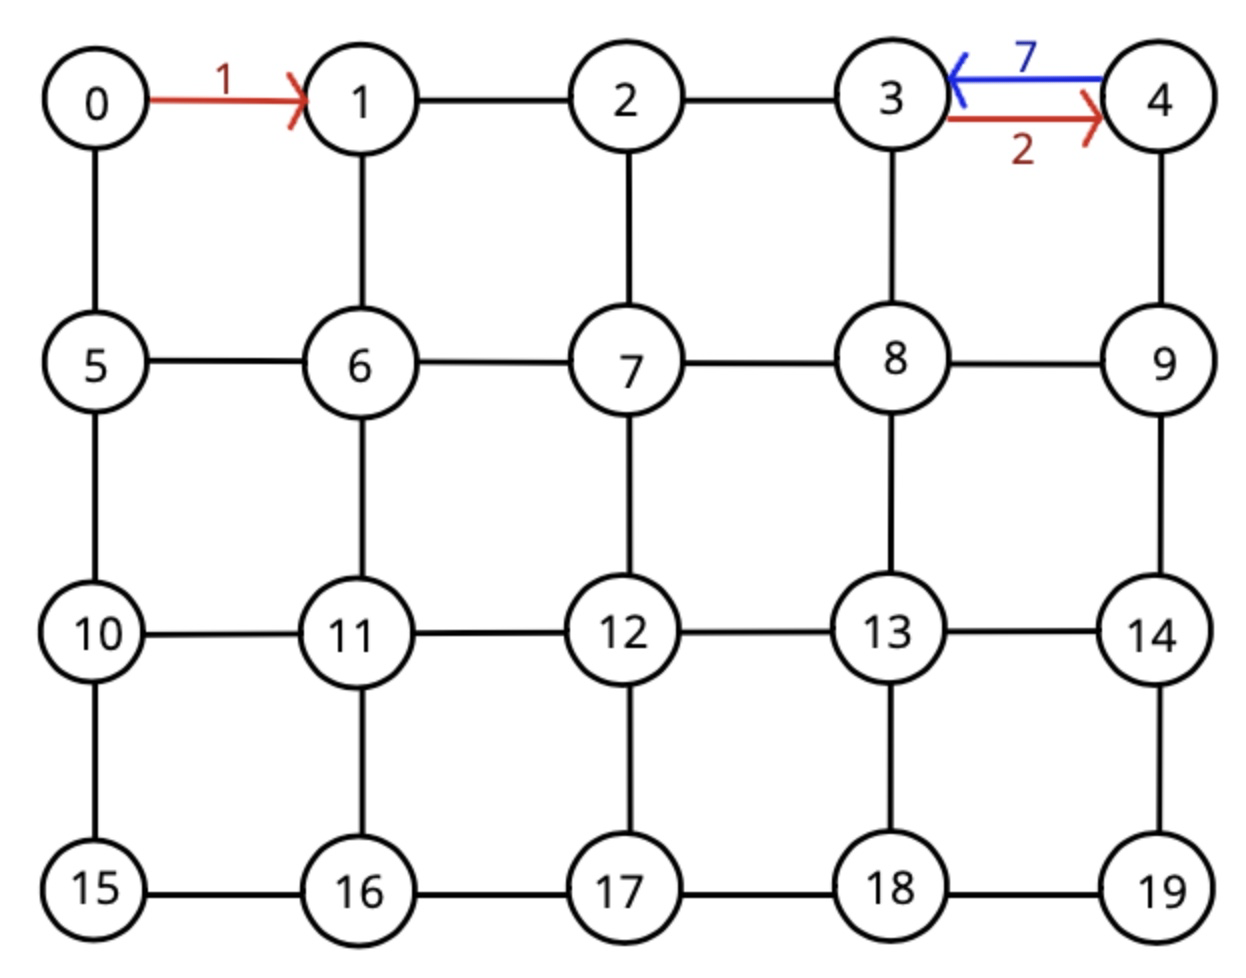
\includegraphics[scale=0.15]{graf}
        \caption{Przykład grafu typu "kratka w kratkę"}
    \end{center}
\end{figure}
\newpage

%sekcja 2
\section{Struktura głównego folderu}
Projekt składa się z jednego folderu głównego \textit{Grapher}, podfolderu \textit{src} oraz
pliku \textit{makefile}. 
Plik makefile odpowiada za pół-automatyczną kompilację całego projektu, natomiast w folderze \textit{src} są pliki \textit{*.c} z kodem źródłowym
oraz pliki nagłówkowe \textit{*.h}. Skompilowanie programu polega na użyciu komendy \textit{make}. Po jej użyciu program będzie posiadał następującą strukturę: 
\newline\newline
%rysowanie struktury
\begin{forest}
    for tree={
      grow'=0,
      child anchor=west,
      parent anchor=south,
      anchor=west,
      calign=first,
      edge path={
        \noexpand\path [draw, \forestoption{edge}]
        (!u.south west) +(7.5pt,0) |- node[fill,inner sep=1.25pt] {} (.child anchor)\forestoption{edge label};
      },
      before typesetting nodes={
        if n=1
          {insert before={[,phantom]}}
          {}
      },
      fit=band,
      before computing xy={l=15pt},
    }
    %opisanie struktury
    [\texttt{Grapher}
        [\texttt{bin}
            [\texttt{*.o}]
        ]
        [\texttt{src}
            [\texttt{*.c}]
            [\texttt{*.h}]
        ]
        [\texttt{makefile}
        ]
        [\texttt{grapher}
        ]
    ]
\end{forest}
\newline W folderze \textit{bin} będą przechowywane pliki maszynowe \textit{*.o}, a plik \textit{grapher} będzie odpowiedzialny za uruchomienie proogramu.

%sekcja 3
\section{Wywołanie Programu}
Program stworzony pod pracę z konsolą systemy Linux (przykładowa dystrybucja: Debian 11.0).

\subsection{Skladnia dla trybów Wage, Edge oraz Random}
Program uruchamiamy za pomocą komendy:
\newline\newline \texttt{./grapher [tryb] [Plik] [Wiersze] [Kolumny] [Poczatek] [Koniec]}
\newline\newline Niezbędne do uruchomienia programu jest podanie wszystkich argumentów wywołania.


\subsection{Składnia dla trybu Read}
\texttt{./grapher [tryb] [Plik] [Flaga] [punkt1] [punkt2] ... [punkt(n)] [punkt(n+1)]}
\newline\newline Niezbędne do uruchomienia programu jest pdoanie przynajmniej pierwszych 5 argumentów wywołania nie licząc nazwy programu. 
\newline\newline Poszczególne elementy składni wszystkic trybów wyjaśniamy w podrozdziale 3.4.
\newpage

\subsection{Format pliku dla trybu Read Mode}
Program do działania w trybie Read Mode przyjmuje plik o określonych właściwościach:
\begin{itemize}
    \item W pierwszym wierszu pliku znajduje się informacja o liczbie wierszy i kolumn jakie składają się na graf,
    \item W każdym następnym wierszu znajduję się informacja o tym z jakimi innymi wierzchołkami połączony jest dany wierzchołek oraz waga jaka odpowiada temu połączeniu.
\end{itemize}
Ze względu na numerowanie wierzchołków od zera, numer wiersza odpowiada numerowi wierzchołka zwiększonego o jeden. 
\newline\newline Przykładowa zawartość pliku:

\begin{lstlisting}
3 3
     1 :0.33  3 :2.32
     2 :3.21
     1 :5.11  5 :2.46
     0 :0.89  4 :3.23  6 :2.21
     1 :1.23  3 :3.27  5 :2.25 7:5.12
     4 :2.33
     3 :3.63  7 :1.22
     6 :6.21  4 :1.34
     5 :4.26  7 :8.1 
\end{lstlisting}

\subsection{Argumenty wywołania programu}
Poniżej wyjaśniamy wszystkie potrzebne argumenty wywołania programu:
\begin{enumerate}
    \item \texttt{[Tryb]:}
    \newline Działanie poszczególnych trybów opisane są w celu projektu, flagi do poszczególnych trybów:
    \begin{itemize}
        \item \textit{-WM} -- Wage Mode
        \item \textit{-EM} -- Edge Mode
        \item \textit{-RM} -- Random Mode
        \item \textit{-ReM} -- Read Mode
    \end{itemize}

    \item \texttt{[Plik]:}
    \newline Plik, do którego zostanie zapisany wygenerowany przez program graf, 
    plik będzie zawsze nadpisywany nową zawartością. W trybie \textit{Read Mode} będzie to plik do czytania.

    \item \texttt{[Wiersze]:}
    \newline Liczba wierszy jakie zostaną wygenerowane w grafie. Liczba ta musi być większa od zera.

    \item \texttt{[Kolumny]:}
    \newline Liczba kolumn jakie zostaną wygenerowane w grafie. Liczba ta musi być większa od zera.

    \item \texttt{[Poczatek]:}
    \newline Początek przedziału z jakiego będą generowane wagi dla krawędzi między wierzchołkami. Musi to być wartość większa od 0.

    \item \texttt{[Koniec]:}
    \newline Koniec przedziału z jakiego będą generowane wagi dla krawędzi między wierzchołkami. Musi to być wartość większa od 0.

    \item \texttt{[Flaga]:}
    \newline Flagi mogą być złożone zarówno z dużych jak i małych liter. Wymaganą flagę wybieramy spośród niżej wymienionych:
    \begin{itemize}
        \item \texttt{-standard} – flaga pozwalająca na wyświetlenie skróconej wersji najkrótszej ścieżki między dwoma zadanymi punktami.
        \newline Format wyświetlania: (od,do); od $\rightarrow$ następny punkt $\rightarrow$ ... $\rightarrow$ do
        \newline \textbf{np.}
        \newline(7,8); 7 $\rightarrow$ 6 $\rightarrow$ 5 $\rightarrow$ 9 $\rightarrow$ 8,
        \item \texttt{-extended} -- flaga pozwalająca na wyświetlenie rozszerzonej wersji najkrótszej ścieżki między dwoma zadanymi punktami.
        \newline Format wyświetlania: (od,do); (od,do); od(waga przejścia) $\rightarrow$ następny punkt(waga przejścia) $\rightarrow$ ... $\rightarrow$ do
        \newline \textbf{np.}
        \newline (7,8); 7(0,4) $\rightarrow$ 6(0,2) $\rightarrow$ 5(0,3) $\rightarrow$ 9(0,1) $\rightarrow$ 8.
    \end{itemize}

    \item \texttt{[Punkt(n)]:}
    \newline Punkt \textbf{od}, którego szukamy drogę w grafie.

    \item \texttt{[Punkt(n+1)]:}
    \newline Punkt \textbf{do}, którego szukamy drogę w grafie.
\end{enumerate}

\subsection{Przykładowe wywołanie programu}
\begin{enumerate}
    \item \textbf{Wywołanie dla składni trybów Wage, Edge, Random}
    \newline Poniżej prezentujemy przykładową komendę wywołania dla trybu Wage mode z poprawnymi danymi. Wybraliśmy tryb Wage Mode, podaliśmy plik, liczbę wierszy i kolumn oraz zakres losowania wag.
    \newline\newline \textbf{np.}
    \newline \texttt{./grapher -WM mygraph 3 5 1 6}
    \newline\newline Wywołanie dla złych danych, tutaj nie podamy pliku:
    \newline\newline \textbf{np.}
    \newline \texttt{./grapher -WM}
    \newline\newline Program udzieli informację o braku podania pliku oraz wyświetli poprawną składnię.
    \newpage
    \item \textbf{Wywołanie dla składni trybu Read}
    \newline Poniżej podaliśmy poprawną komendę wywołania dla trybu Read. Wybraliśmy tryb, podaliśmy plik, flagę oraz podaliśmy punkty od i do, którego szukamy najkrótszej ścieżki.
    \newline\newline \textbf{np.}
    \newline \texttt{./grapher -ReM mygraph -standard 7 8}
    \newline\newline Wynikiem działania programu będzie wyświetlenie najkrótszej ścieżki. 
    \newline Tutaj przedstawiamy przykład wywołanie progamu bez flagi:
    \newline\newline \textbf{np.}
    \newline \texttt{./grapher -ReM mygraph }
    \newline\newline Program wyświetli komunikat o braku flagi i składnię programu.
\end{enumerate}

%sekcja 4
\section{Wyjście programu}
Program zapisuje strukturę wygenerowanego grafu do pliku oraz wypisuje na konsolę informacje o wyniku swojego działania.
\newline W zależności od trybu na konsoli zostanie wyświetlona informacja:

\begin{itemize}
    \item Wage Mode -- o pomyślnym wygenerowaniu grafu,
    \item Edge Mode – o wygenerowaniu grafu spójnego jeśli uda się to wykonać poniżej 500 prób, w przeciwnym wypadku program zapyta użytkownika czy chce kontunować losowanie krawędzi i wag,
    \item Random Mode – o tym czy graf jest spójny, a następnie poda plik do którego go zapisał,
    \item Read Mode -- o spójności grafu i w przypadku odczytania grafu spójnego o najkrótszej ścieżce między zadanymi punktami.
\end{itemize}
Wszelkie komunikaty o błędach zostają wypisane na konsolę, wraz z instrukcją dotyczącą składni programu.

%sekcja 5
\section{Obsługiwane błędy}
W poniższej tabeli wypisaliśmy błędy jakie mogą wystąpić w czasie działania programu oraz wyjaśniliśmy co znaczą.

%wyświetlanie tabeli
\begin{tabularx}{\textwidth}{ l|c|l } 
\hline Nazwa Błędu & Kod & Wyjaśnienie błędu\\ 
\hline NO\_MODE\_FOUND & 501 & Niepoprawny tryb lub jego brak\\ 
\hline NO\_FILE\_FOUND & 502 & Nie podano pliku lub plik nie istnieje\\ 
\hline WRONG\_NUM\_OF\_ROWS & 503 & Podano niepoprawną liczbę wierszy\\
\hline WRONG\_NUM\_OF\_COL & 504 & Podano niepoprawną liczbę kolumn\\
\hline WRONG\_RANGE\_OF\_WAGES & 505 & Zły zakres losowania wartości wag\\
\hline NO\_FLAG\_FOUND & 611 & Nie podany flagi w trybie Read Mode\\
\hline WRONG\_POINTS & 612 & Podano nieistniejący punkt lub ich złą liczbę\\
\hline NO\_COHERENT & 613 & Graf jest niespójny \\
\hline
\end{tabularx}

\end{document}